% !TEX encoding = UTF-8 Unicode
% !TEX TS-program = pdflatex
\newif\ifprint % to compile the print version or the digital one
\printtrue     % to compile the print version
\printfalse    % to compile the digital version  (default) - comment this line to compile the print version
% toptesti document class
\documentclass[%
    a4paper, % not needed, by default it is a4paper, or also b5paper can be used
    corpo=12pt, % dimension of basic font
    % oneside is generally the way to go
    oneside, % two side optimizes for two-face printing, having chapters open on the right (aka odd numbers), if you don't want blank pages put oneside here
    stile=standard,
    %evenboxes, % not needed, to put supervisors and candidate at the same level
    tipotesi=magistrale,
    numerazioneromana, % roman numbering for appendixes and preambles, up to Table of Contents
    openright, % to force opening on the right for double-sided printing
    cucitura=0mm, % for printing, 7mm should be enough
    %draft,
    %dvipsnames, % for compatibility with xcolor, it does not work
]{toptesi}

\input{common/packages}
\input{common/package_config}

% how to change Contents to Table of Contents
\addto\captionsenglish{% Replace "english" with the language you use
  \renewcommand{\contentsname}%
    {Table of Contents}%
}

% to change the name of Abbreviations to Acronyms
% not needed if use use entry types and define those
% \renewcommand{\abbreviationsname}{Acronyms}

% to allow line comments in algorithms
\algnewcommand{\LineComment}[1]{\State \(\triangleright\) #1}

% to declare abs and norm
\DeclarePairedDelimiter\abs{\lvert}{\rvert}%
\DeclarePairedDelimiter\norm{\lVert}{\rVert}%

% Swap the definition of \abs* and \norm*, so that \abs
% and \norm resizes the size of the brackets, and the 
% starred version does not.
\makeatletter
\let\oldabs\abs
\def\abs{\@ifstar{\oldabs}{\oldabs*}}
%
\let\oldnorm\norm
\def\norm{\@ifstar{\oldnorm}{\oldnorm*}}
\makeatother

%% *** ARIEL PRIARONE ***
\let\dummy\autoref % This redefine autoref as dummy
\def\autoref#1{\textbf{\dummy{#1}}} % this is like \autoref but in bold
\newcommand{\algorithmautorefname}{algorithm} % to make autoref work with algorithms
\addto\extrasenglish{\def\figureautorefname{figure}}%
\addto\extrasenglish{\def\chapterautorefname{chapter}}%
\addto\extrasenglish{\def\sectionautorefname{section}}%
\addto\extrasenglish{\def\subsectionautorefname{subsection}}%
\addto\extrasenglish{\def\subsubsectionautorefname{subsubsection}}%
\addto\extrasenglish{\def\paragraphautorefname{paragraph}}%
\addto\extrasenglish{\def\tableautorefname{table}}%
\addto\extrasenglish{\def\equationautorefname{equation}}%

\newcommand{\vect}[1]{\bm{#1}}  % for vectors
\newcommand{\quoted}[1]{``#1''} % for quotes
\newcommand{\argmin}[1]{\mathrm{arg}\,\underset{#1}{\mathrm{min}}}
\newcommand{\argmax}[1]{\mathrm{arg}\,\underset{#1}{\mathrm{max}}}
\newcommand{\citepage}[2]{\cite[p.~#2]{#1}}

\DeclareMathOperator*{\E}{\mathbb{E}}

\colorlet{punct}{red!60!black}
\definecolor{delim}{RGB}{20,105,176}
\colorlet{numb}{magenta}
\definecolor{eclipseStrings}{RGB}{42,0.0,255}
\definecolor{eclipseKeywords}{RGB}{0,100,0}
\lstdefinelanguage{json}{
    basicstyle=\scriptsize\ttfamily,
    commentstyle=\color{eclipseStrings}, % style of comment
    stringstyle=\color{eclipseKeywords}, % style of strings
    numbers=left,
    numberstyle=\scriptsize,
    stepnumber=1,
    numbersep=8pt,
    showstringspaces=false,
    breaklines=true,
    frame=lines,
    string=[s]{"}{"},
    comment=[l]{\#},
    morecomment=[l]{:"},
    literate=
        *{0}{{{\color{numb}0}}}{1}
         {1}{{{\color{numb}1}}}{1}
         {2}{{{\color{numb}2}}}{1}
         {3}{{{\color{numb}3}}}{1}
         {4}{{{\color{numb}4}}}{1}
         {5}{{{\color{numb}5}}}{1}
         {6}{{{\color{numb}6}}}{1}
         {7}{{{\color{numb}7}}}{1}
         {8}{{{\color{numb}8}}}{1}
         {9}{{{\color{numb}9}}}{1}
}



\newcommand{\mask}[1]{#1} % to mask text
\newcommand{\maskk}[1]{} % to mask text in introduction
\newcommand{\maskkk}[1]{#1} % decide where to put this paragraph
\newcommand{\maskglossaries}[1]{} % to mask glossaries
\input{common/thesis_info.tex}
\input{common/font_config.tex}

\addbibresource{bibliography.bib}

% % to load the glossaries, not needed if using bib2gls
 % for glossary entry
% @entry{bird,
%     name={bird},
%     description = {feathered animal},
%     see={[see also]{duck,goose}}
% }

% if this bib file does not work, try using \input{file.tex}
% where all the \newabbreviation commands have been inserted
% containing all the definitions

% Gls to capitalize first letter
% GLS for full uppercase
% for abbreviations also
% glsxtrshort for abbreviation
% similar for long, full, and capital configurations, add pl at the end for plurals
% glsentryshort, long, plural (referred to shorts) must be used when in section titles
% glslink to allow the link but use a different text (as for href)


% if you want to use also description for the abbreviations/acronyms, you should use bib2gls and define all the entries in a bib file, which is incompatible with Overleaf
\newacronym{lcm}{LCM}{Least Common Multiple}
\newacronym{pm}{PM}{Predective maintenance}
\newacronym{AI}{AI}{Artificial intelligence}
\newacronym{pdm}{PdM}{Predictive Maintenance}
\newacronym{rm}{RM}{Reactive Maintenance}
\newacronym{aka}{a.k.a.}{Also Known As}
\newacronym{pof}{POF}{Pareto Optimal Front}

%Symbols
\glsxtrnewsymbol[
    description={\textbf{Cluster} A set of objects that are more similar to each other than to those in other clusters.}]
    {sym:cluster}
    {\ensuremath{\vect{\mathcal{C}}}}

\glsxtrnewsymbol[
    description={\textbf{Snapshot} A set of features that describe the state of a system at a given time.}]
    {sym:snap}
    {\ensuremath{\vect{\mathcal{S}}}}
    
\glsxtrnewsymbol[
    description={\textbf{Snapshots Set} A set of snapshots \gls{sym:snap}.}]
    {sym:snapset}
    {\ensuremath{\vect{\mathbf{S}}}}

%Glossary
\newglossaryentry{ex}{name={example},description={an example}}
\newglossaryentry{cow}{name={cow},plural={cows},description={an adult female of any bovine animal.}} 
\newglossaryentry{par}{name={paragraph},description={distinct section of a piece of writing}}





 \makeglossaries
 \label{glossary}

\begin{document}

\input{common/config}

\input{common/toptesi_config}

% front page
% frontespizio can be used for the first page print
% while the custom-made frontpage can be used as hard-cover
% use pdfjoin or pdfseparate to extract or put together the pages if needed
%\frontespizio* % without star the logo is on top
\input{common/frontpage.tex} % custom frontpage
%\retrofrontespizio
% insert text for the back of the front page
% if you insert any remove the following \paginavuota
% either a blank page or a back is needed to have double-sided printing
% pay attention to leave the space for the page

%\paginavuota % clears a page

\frontmatter

% abstract if needed
% \begin{abstract}
%     \gls{glo:predictivemaintenance} and Novelty Detection are important topics in modern industrial engineering, aimed at proactively identifying equipment failures before they affect system functionality. Embracing these practices is crucial for reducing equipment downtime and optimizing maintenance efforts. \gls{glo:predictivemaintenance} aims to quantify and forecast the state of degradation of a system. A quite novel frontier is the direct implementation of \gls{glo:predictivemaintenance} within the maintained device, using the principles of Edge Computing.

The fourth industrial revolution is characterized by the integration of Artificial Intelligence and the Internet of Things paradigm into factories. Nowadays, more than a decade since the beginning of this industrial revolution, the maintenance approach remained unchanged in most industrial applications. The primary factor impeding the advancement of the maintenance approach is the significant expense associated with implementing Condition-Based or Predictive maintenance strategies, coupled with a lack of knowledge about the modelling or behaviour of a failing system.

In most facilities, maintenance continues to be performed according to a predefined schedule. An optimization of this approach involves intervening in the system only when necessary, which requires the knowledge of when a system is malfunctioning. Fault Detection and Novelty Detection enable triggering an event when a known fault occurs or when a new, unfamiliar behaviour emerges in the maintained system. 

In this thesis, a \gls{glo:frmwrk} that performs Novelty Detection is proposed. The structure of the \gls{glo:frmwrk} is thought to be modular and general-purpose to ease the implementation into different systems. It is developed following an Unsupervised Machine Learning approach to overcome the common lack of physical models of the maintained device. The Machine Learning core of the \gls{glo:frmwrk} is based on the \gls{glo:feature}s extracted from the data gathered from sensors. In the first phase, the data are used to train the models. Then, the \gls{glo:frmwrk} operates in real time, continuously assessing the status of the system. This solution provides a novelty metric that estimates how unfamiliar the current state of the system is and a forecast of the future evolution of the system.

Firstly, it has been developed to be executed and tested on a \gls{pc} using various Unsupervised Machine Learning algorithms. The algorithm that appeared to better balance performance and hardware resource consumption was deployed on a microcontroller. The proposed solution includes all the tools necessary in the data pipeline. Relying on the general-purpose structure proposed, the \gls{glo:frmwrk} can be easily set up on a machine and extended to an arbitrary configuration of sensors and \gls{glo:feature}s. 

The \gls{pc} implementation underwent testing using various Unsupervised algorithms on publicly available datasets, while the edge implementation was tested through laboratory experiments.

Both the tests on datasets and the experimental results showed that the proposed \gls{glo:frmwrk} is able to detect novelties and give an estimate of the future evolution of the novelty metric of the system.
% \end{abstract}

% to create blank pages for openright in frontmatter
% use one of the following two methods
% 1) use the following three lines
%\phantom{0} % needed otherwise cleardoublepage does not clean the page because it sees it empty
%\cleardoublepage
%\thispagestyle{empty} % to have empty page, without numbers
% 2) or

\ifprint \customClearDoublePage \fi % to have a blank page and start on a fresh right page
\includegraphics[height=.95\textwidth,angle=90,origin=c]{images/wordcloud_svg-raw.pdf}

\ifprint \customClearDoublePage \fi % to have a blank page and start on a fresh right page
\ifprint \else \ringraziamenti  \fi% acknowledgements

\ifprint \vspace*{10\baselineskip} \else
{I would like to thank the PoliTO Interdepartmental Centre for Service Robotics (PIC4Ser) for giving me the opportunity to work on this project. The guidance and infrastructure provided by the centre have been invaluable during the development of this work.
\vspace*{5\baselineskip}}
\fi

\begin{flushright}
    To my parents, who have given me everything.\\
    Thank you for always making me believe that nothing is impossible.\\
    \textit{{Ai miei genitori, che mi hanno dato tutto.\\ 
    Grazie per avermi sempre fatto credere che niente sia impossibile.}} \\[\baselineskip]
    \textit{Ariel}
\end{flushright}


\ifprint \customClearDoublePage \fi % to have a blank page and start on a fresh right page


\maskabstract{
%\fontsize{11}{13.6}\selectfont{
\sommario\input{
    content/Abstract.tex
%    }
    }} % abstract

{\ifprint \customClearDoublePage \fi
\pdfbookmark[0]{\contentsname}{toc}%
\tableofcontents}

\listoftables % ToC for tables

\listoffigures % ToC for figures

% actually abbreviation is the name used for acronym in glossaries-extra
% title sets the name
% type tells the type of glossary to print
% style overrides the global style
% here we are printing only abbreviations
% printunsrtglossary if using record, otherwise printglossary is ok

%\printunsrtglossary[style=altlist,title=Acronyms,type=\glsxtrabbrvtype] % A.P. rimosso perchè toptesi fa schifo
\maskglossaries{\printglossaries}

% also list of symbols here if needed

\input{common/post_summary_config.tex} 

\mainmatter

%\part{Prima Parte} % parts division, not needed
% Chapters always open on a right-side page, i.e. odd numbers, so a blank page is inserted if needed
%\cleardoublepage[empty] % to have a fully blank page
% a blank page appears before the first chapter in some configurations, on the last version it doesn't

% list here all the chapters
\chapter{Introduction}
\label{ch:introduction}

{\section{Preface}
\label{sec:preface}

Imagine being the owner of a piece of technology. It can be any physical device. Without maintenance, it is unavoidable that, after a certain amount of time of usage it will have some sort of malfunction.
To overcome this problem, usually, maintenance work is planned and performed by a team of skilled technicians. 

The simplest way of executing maintenance is to fix the device when it breaks. This is called \emph{reactive maintenance} (\gls{rm}). This has been done since forever, and it is still a very popular approach today, but it has a lot of drawbacks, ranging from the high downtime for repair, and the logistics of the spare parts etc.

The other family of maintenance techniques is called \emph{preventive (or proactive) maintenance} (\gls{pvm}). All those techniques share the property of being applied before the device shows a malfunction. This is a very broad category, and it includes a lot of different techniques, most of which will be described in this thesis.

Back to the example, the owner of the device may want to avoid fixing it when it has already failed as much as possible, so the first improvement could be to perform maintenance periodically (on a schedule). This is called \emph{predetermined maintenance}. It's basically the same approach that every car owner uses to minimize the risk of the vehicle breaking down in the middle of the road. 
The owner may want to take the technique a step further and seek some sort of guidance on deciding when to perform maintenance. A very intuitive approach is to simply ask the skilled technicians to inspect all the devices very often to try to understand if something is wrong without interfering with the normal operation of the device.

If a technician has enough experience, he may be able to detect the vast majority of the problems before they become critical. He may do that simply using his senses, for example by listening to the sound of the device, or by touching it to feel how much it vibrates, how hot is it and so on. 

\maskk{I would like to share, as a real-life example, what I witnessed during the commissioning of a new power plant. I remember that the commissioning manager (that is a chemist) was able to detect if the demineralization unit was working properly or not by simply tasting the water it produced, before the necessary instruments were installed.}

This naive approach can be enhanced by using a large number of sensors to monitor the most critical parameters of the device. In this case, the technician will train himself more on the data of the sensors, rather than on inspecting the device directly. 

At this point, the next logical step would be to use the data from the sensor to train an algorithm, that will detect some patterns in the data that are not easily detectable by a human. This is called \emph{condition-based maintenance} (\gls{cbm}). This is the most common approach to \gls{pm} today. If this algorithm is trained only on the data taken when the device is working properly, it would only be able to detect a novel behavior, this is called \emph{novelty detection} (\gls{nd}). If the algorithm is trained on both the data taken when the device is working properly and the data taken when the device is malfunctioning in a specific way, it would be also able to detect the specific malfunction, this is called \emph{fault detection} (\gls{fd}).

One last improvement to the \gls{cbm} approach is to use an algorithm that will also try to predict how much time is left before a critical malfunction will occur. This approach is referred to as \emph{predictive maintenance} (\gls{pdm}). This is the most advanced approach to \gls{pm} today.

Both \gls{cbm} and \gls{pdm} could be done by using a model of the system that will predict the future behavior based on the current state of the system. The problem with this approach is that it is very difficult to build a model that is accurate enough to be useful. Most of the time, in industrial application, such a model is not available.
A workaround to this problem is to apply an Unsupervised Machine Learning (\gls{uml}) algorithm to the sensors data. This has the advantage of not needing a model of the system, but it has the drawback of being a black-box approach, so the parameters of the algorithm are not easily interpretable in a phisical sense. Furthermore, the algorithm will be fairly good at detecting anomalies, but it will have some limitations in predicting the future behavior of the system, since it will likely be based on a forecast done interpolating the data of the past.

\paragraph*{}
To visualize this evolution of maintenance approaches, let's have a look to \autoref{fig:earlysteamengine}. This is a purely mechanical device, so the only way to detect a malfunction before it causes a failure is by trusting the \quoted{gut feeling} of the operator. Moving on, the device in \autoref{fig:modernsteamengine} is also a steam engine, but it is equipped with some analogue gauges. In this case is it possible to define some thresholds for the readings that are indicative of a malfunction and look at the time evolution of the values. The measure of the sensor is immediatly displayed to the operator. Moving into present days, the device in \autoref{fig:controlroom} is a state of the art control room. The data from the sensors are elaborated by a computer and displayed to the operator on screens. This allows the computer to run algorithms on the sensor data.

\begin{figure}
    \centering
    \begin{subfigure}{0.3\textwidth}  % <----
        \includegraphics[width=\textwidth]{images/Intro/earlysteamengine.jpg}
        \caption{early steam engine \cite{steam_engine}}
        \label{fig:earlysteamengine}
    \end{subfigure}
    \begin{subfigure}{0.3\textwidth}  % <----
        \includegraphics[width=\textwidth]{images/Intro/modernsteamengine.jpg}
        \caption{steam engine \cite{triple_expansion_engine}}
        \label{fig:modernsteamengine}
    \end{subfigure}
    \begin{subfigure}{0.3\textwidth}  % <----
        \includegraphics[width=\textwidth]{images/Intro/control-rooms-workstations.jpg}
        \caption{control room \cite{evosite}}
        \label{fig:controlroom}
    \end{subfigure}
    \caption{Evolution of machinery}
    \label{fig:machineryevolution}
\end{figure}

\paragraph*{}
The last comment is about where to run the algorithm. The most common approach is to run it un a server, that is not part of the device itself. This has the adventage of not having constraint on how much computational power is needed, because it's usually feasible to add more computational power to a computer that is not located on the device itself. The main drawback is that the data have to be transmitted to the server. This may not be feasible in some cases, for example for a mobile device, or for a device that is located in a remote area with no internet connection. In this case, the algorithm has to be run near the device itself, usually on a microcontroller that will perform an action when the algorithm detects a malfunction. This approach is called \emph{\gls{glo:edge}}. Using a microcontroller also has the advantage of using very little power, this is critical for battery-powered devices.


}
{\section{Motivation}
\label{sec:motivation}

\begin{figure}
    \centering
    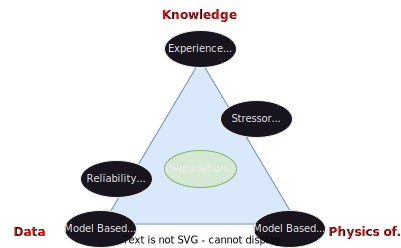
\includegraphics[scale=1.3]{images/Intro/MaintTriangle.pdf}
    \caption{Maintenance triangle}
    \label{fig:MaintTriangle}
\end{figure} 

Takin as example a survay published by the U.S. Department of Commerce in 2020, the maintenance expenditure of the manufacturing industry in the United States were \$57.3 billion, while the losses due to preventable maintenance issues amounted to \$119.1 billion. The top 25\% of those 
establishments relying on reactive maintenance was associated with 3.3 times more downtime 
than those in the bottom 25\% \cite{NIST}. This means that the economic impact of failures exceeds the cost of maintenance by a factor of 2.1, and this is concentrated on those sectors that rely more on reactive maintenance. This emphasizes the importance of developing a general purpose \gls{pdm} system that can be applied in a large variety of systems.

In the article \cite{Maintenance_cat}, the authors divide the \gls{cbm} strategies in five categories:

\begin{itemize}
    \item ccc%\emph{experience based} predictions are based on the experience and knowledge outside or within the company. It is based on little scattered data on average conditions. The only  requirement is that the experience of the experts is quantified and used;
    \item \emph{reliability statistics} predictions are based on the statistical analysis of the failure data without considering the specific system. These methods also estimate the life
    of an average component operating under historically average conditions;
    \item \emph{stressor based} predictions can be considered an extension of the reliability statistics methods. The difference is that they also consider a measure of the stress (humidity, temperature, etc.) that the component is exposed to;
    \item \emph{degradation based} predictions are based on the extrapolation of the degradation of the component;
    \item \emph{model based} predictions are based on the knowledge of the physics of the system. The assumption is that the degradation can be computed instead of meadured. They can be based on a physical model or on a data-driven model.
\end{itemize}


The authors of \cite{Maintenance_cat} also propose a distribution of this categories in a triangle, as shown in \autoref{fig:MaintTriangle}. Each vertex of represent a requisite for the implementation, and the distance of the method to the represent how dependent it is on that requisite. To obtain a general purpose \gls{pdm} framework, the \emph{degradation based} approach seems the most promising, since it is the least dependent on a specific requisite.

Moreover, to enhance even more the general purpose nature of the framework, a \gls{uml} model has been implemented in the framework. This speed up the implementation of the framework on a machine about which little is known, plus, it can be implemented on a new machine without a deep knowledge of the \gls{uml} algorithm themeself.

In the paper \cite{GridPredictMaintenance}, it is pointed out that \gls{glo:edge} implementations, not only enable the use of the framework for special aplications, but it also enhance the cybersecurity of facilities may not need an edge implementation because of technical limitations.}
{\section{Objective of the thesis}
\label{sec:objectives}

The goal of this thesis is to design, code and test an algorithm that will perform \gls{nd}, \gls{fd} and \gls{pdm}. This algorithm will be implemented twice:
\begin{itemize}
    \item  coding in \texttt{python} and running it on a \gls{pc};
    \item   coding in \texttt{C} and running it on a microcontroller.
\end{itemize}

To do that }
{\section{Notations}
\label{sec:notations}
In this thesis, the following notations are used:
\begin{itemize}
  \item bold lowercase letters ($\vect{a}$, $\vect{b}$, $\vect{c}$) are used to denote vectors;
  \item italic lowercase letters ($a$, $b$, $c$) are used to denote scalars;
  \item bold uppercase letters ($\vect{A}$, $\vect{B}$, $\vect{C}$) are used to denote matrices;
  \item $\vect{a}_{i(j)}$ is the $j$th element of the vector $\vect{a}_i$;
  \item $||\vect{a}||_2$ is the $l^2$-norm of the vector $\vect{a}$, defined as $\sqrt{\sum_{i=1}^{n} a_i^2}$, denoted also as $\norm{a}$ for simplicity;
  \item $||\vect{a}||_n$ is the generic $l^n$-norm of the vector $\vect{a}$, defined as $\sqrt[n]{\sum_{i=1}^{n} \abs{a_i}^n}$;
  \item parenthesis encapsulating an index are used to condense descriptions, for example \quoted{\textbf{$\vect{a}_{i(j)}$ is the force applied to the $i$th ($j$th) step}} means that $\vect{a}_i$ is the force applied to the $i$th step and $\vect{a}_j$ is the force applied to the $j$th step;
\end{itemize}

No distinction in notation is made between a vector in the phisycal sense (applied to a point, with a direction, and a magnitude) and a vector in the mathematical sense (a generic number $\in \mathbb{R}^n $).
}
\ifprint \section{Licence}
\label{sec:licence}

\subsection{This document Licence}
The content of this thesis is released under the Creative Common Attribution-NonCommercial-NoDerivatives 4.0 International ({CC BY-NC-ND 4.0})\footnote{\url{https://creativecommons.org/licenses/by-nc-nd/4.0/}}. 

You are free to copy and redistribute the material in any medium or format, under the following terms:
\begin{itemize}
    \item \includegraphics[width=12pt]{images/CreativeCommons/by.eps}\textbf{ Attribution} - You must give appropriate credit , provide a link to the license, and indicate if changes were made . You may do so in any reasonable manner, but not in any way that suggests the licensor endorses you or your use.
    \item \includegraphics[width=12pt]{images/CreativeCommons/nc-eu.eps}\textbf{ NonCommercial} - You may not use the material for commercial purposes 
    \item \includegraphics[width=12pt]{images/CreativeCommons/nd.eps}\textbf{ NoDerivatives} - If you remix, transform, or build upon the material, you may not distribute the modified material.
    \item \textbf{No additional restrictions} - You may not apply legal terms or technological measures that legally restrict others from doing anything the license permits.
\end{itemize}

You do not have to comply with the license for elements of the material in the public domain or where your use is permitted by an applicable exception or limitation .

No warranties are given. The license may not give you all of the permissions necessary for your intended use. For example, other rights such as publicity, privacy, or moral rights may limit how you use the material.

\begin{figure*}
    \centering
    \includegraphics{images/CreativeCommons/by-nc-nd.eu.pdf}
\end{figure*}

\subsection{Code Licence}
The code used in this thesis is available at \url{https://github.com/arielpriarone/Thesis.git}. The license under which specifically the code is released is visible in the \texttt{github} repository. \fi
\chapter{Clustering}

\section{Evaluation of a new instance}

At this point, with a model trained on the data, a generic $n$th new snapshot instance $\vect{\mathcal{S}}_n$ can be evaluated using the K-means algorithm.
From a geometric point of view, the snapshot $\vect{\mathcal{S}}_n$ is a point in the ${F}$-dimensional space, where ${F}$ is the number of features used to train the model.

For demonstration purposes, in this section, it is considered an example with ${F}=3$ features.

\begin{figure}[htbp]
  \centering
  \includegraphics[width=\textwidth]{images/Spheres_2.pdf}
\caption{Cluster model in the $3$-dimensional space, with new snapshot $\vect{\mathcal{S}}_n$}
\label{fig:clust_spheres}
\end{figure}

In the \autoref{fig:clust_spheres}, the training data are represented in the $3$-dimensional space, where the axis are the features used to train the model. The K-means model has been ideally trained with an arbitrary number $k$ of clusters but, for display purposes, only two clusters  ($\vect{\mathcal{C}}_i$ and $\vect{\mathcal{C}}_j$) are plotted. 
\paragraph*{}
The entities shown in the \autoref{fig:clust_spheres} are:
\begin{itemize}
  \item $\vect{\mathcal{C}}_i$ is the set of training snapshots belonging to the $i$th cluster, it has a centroid $\vect{c}_i$ and a radius $\vect{r}_i$;
  \item $\vect{\mathcal{C}}_j$ is the set of training snapshots belonging to the $j$th cluster, it has a centroid $\vect{c}_j$ and a radius $\vect{r}_j$;
  \item $\vect{\mathcal{S}}_n$ is the new snapshot to be evaluated;
  \item $\vect{d}_{n,i}$ is the distance between $\vect{\mathcal{S}}_n$ and $\vect{c}_i$;
  \item $\vect{d}_{n,j}$ is the distance between $\vect{\mathcal{S}}_n$ and $\vect{c}_j$;
\end{itemize}

\subsection{Assign the new instance to a cluster} 


% \paginavuota % it works even without stile=classica

\appendix
% appendix
\mask{\chapter{Fast Fourier Transform}
\label{app:FFT}
}
\mask{\chapter{Wavelet Transform}
\label{app:wavelet}}


% endnotes here if needed

\customClearDoublePage
\printbibliography[heading=bibintoc] % heading required to show it in ToC

\end{document}
